\documentclass{standalone}
\usepackage{circuitikz,siunitx}
\usetikzlibrary{shadings,decorations.pathmorphing,arrows.meta,patterns}

\begin{document}
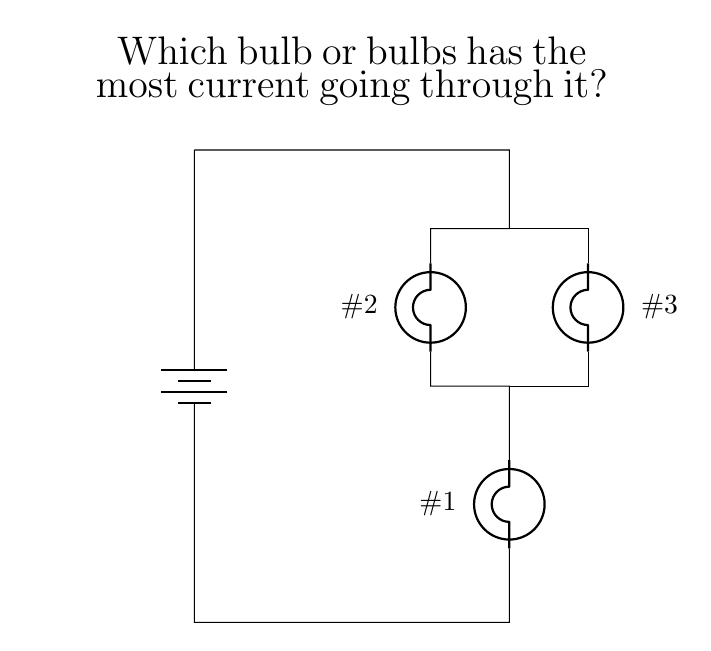
\begin{tikzpicture}
    \draw (-1,6)
      to[battery]                   (-1,0)
      to                             (3,0)
      to[bulb,l={\#1}]             ++(0,3)
      coordinate (j)
      to                          ++(-1,0)
      to[bulb,l={\#2}]             ++(0,2)
      to                           ++(1,0)
      to                           ++(0,1)
      to                            (-1,6)
      ;
    \draw (j)
      to                           ++(1,0)
      to[bulb,l_={\#3}]            ++(0,2)
      to                          ++(-1,0)
      ;             
    \node[align=center,text width=8cm] at (1,7) {\centering \Large Which bulb or bulbs has the most current going through it?};       
\end{tikzpicture}
\end{document}